\documentclass[12pt, polish]{article}
\usepackage[T1]{fontenc}
\usepackage{polski}
\usepackage[utf8]{inputenc}
\usepackage[polish]{babel}
\usepackage{graphicx} 
\usepackage{wrapfig}
\usepackage{sidecap}
\usepackage{subfig}
\usepackage[a4paper,margin=1in,footskip=0.25in]{geometry}

\usepackage{csvsimple,booktabs}
\usepackage{filecontents}
\usepackage{graphicx}

\begin{filecontents*}{data_from_quicksort_better.csv}
ilość elementów, czas[s]
10,1.2e-06
100,2.2e-06
1000,1.7e-05
10000,0.000143
100000,0.0015008
1000000,0.0156854
10000000,0.157468
\end{filecontents*}

\begin{filecontents*}{data_from_quicksort_middle.csv}
ilość elementów, czas[s]
10,1.2e-06
100,4.2e-06
1000,4.54e-05
10000,0.0005718
100000,0.0067092
1000000,0.0780638
10000000,0.876317
100000000,9.88534
\end{filecontents*}

\begin{filecontents*}{data_from_quicksort_worst.csv}
ilość elementów, czas[s]
10,1.4e-06
100,1.36e-05
1000,0.0010008
10000,0.100182
100000,10.0234
\end{filecontents*}

\begin{filecontents*}{data_from_mergesort_better.csv}
ilość elementów, czas[s]
10,1.2e-06
100,4.6e-06
1000,5.56e-05
10000,0.0007434
100000,0.0083426
1000000,0.101612
10000000,1.16551
\end{filecontents*}

\begin{filecontents*}{data_from_mergesort_middle.csv}
ilość elementów, czas[s]
10,1.6e-06
100,5.8e-06
1000,6.6e-05
10000,0.000753
100000,0.0087794
1000000,0.105519
10000000,1.18686
\end{filecontents*}

\begin{filecontents*}{data_from_mergesort_worst.csv}
ilość elementów, czas[s]
10,1.4e-06
100,6.2e-06
1000,6.68e-05
10000,0.0008674
100000,0.0103934
1000000,0.123629
10000000,1.41516
\end{filecontents*}

\begin{filecontents*}{data_from_heapsort_better.csv}
ilość elementów, czas[s]
10,1.2e-06
100,2.2e-06
1000,1.7e-05
10000,0.000143
100000,0.0015008
1000000,0.0156854
10000000,0.157468
\end{filecontents*}

\begin{filecontents*}{data_from_heapsort_middle.csv}
ilość elementów, czas[s]
10,1.6e-06
100,1.16e-05
1000,0.0001552
10000,0.0019166
100000,0.024317
1000000,0.292083
10000000,3.34007
\end{filecontents*}

\begin{filecontents*}{data_from_heapsort_worst.csv}
ilość elementów, czas[s]
10,2e-06
100,1.46e-05
1000,0.000202
10000,0.0023866
100000,0.0296416
1000000,0.36103
10000000,4.55591
\end{filecontents*}

\author{Patrycja Polek \\ Kiełbasa Kamil}
\title{\textbf{PROJEKTOWANIE ALGORYTMÓW I METODY SZTUCZNEJ INTELIGENCJI}}

\begin{document}
\maketitle
\tableofcontents

\newpage
\section{Wstęp}
Celem naszego projektu była implementacja algorytmów sortowanie: QuickSortu, HeapSortu oraz MergeSortu, a także porównanie ze sobą ich złożoności obliczeniowej w różnych przypadkach ułożeń sortowanych elementów. Na podstawie tej wiedzy napisaliśmy algorytm hybrydowy,który stwierdzał jaki rodzaj sortowania zastosować, by czas działania był jak najkrótszy.

\section{Kod źródłowy}

\subsection{Schemat powiązań klas}

\begin{figure}[ht]
	\centering
	\subfloat[Hybridsort]{\label{odnosnik}
		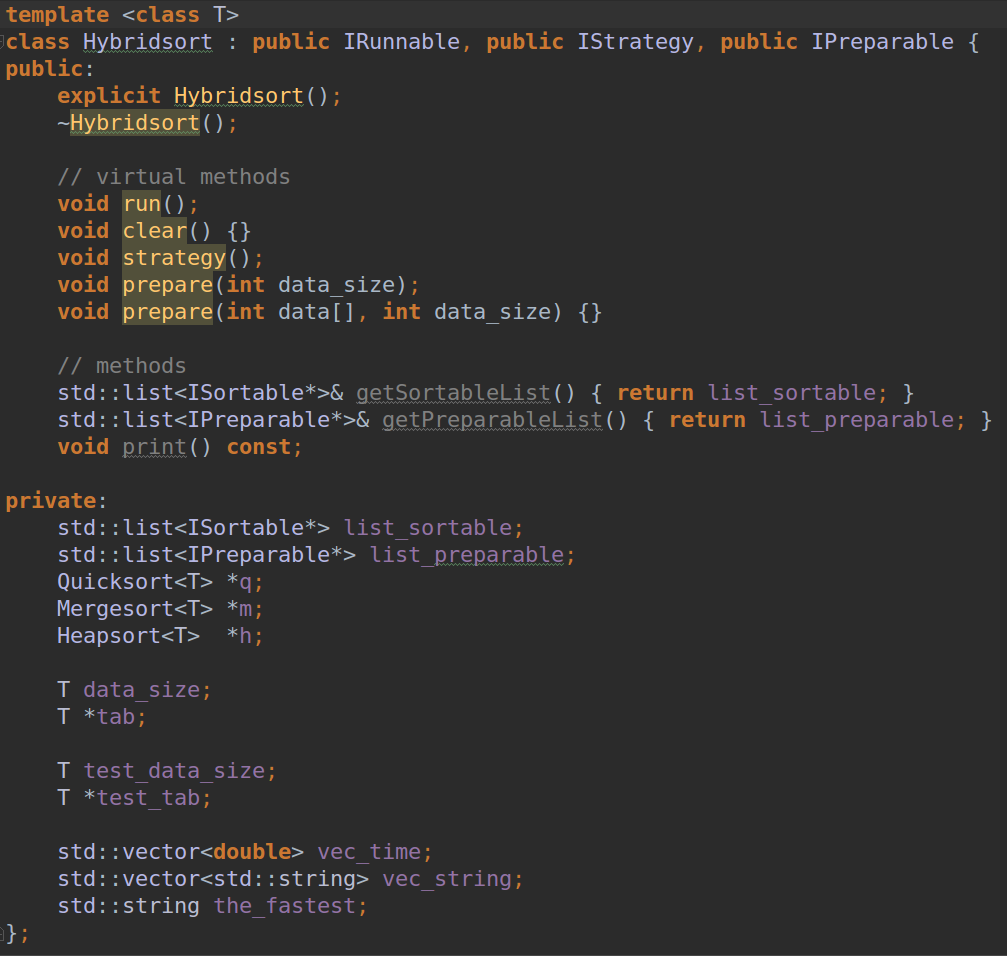
\includegraphics[width=0.6\textwidth]{images/hybridsort.png}}
	\quad
	\caption{Diagram}
\end{figure}

\begin{figure}[ht]
	\centering
	\subfloat[Hybridsort]{\label{odnosnik}
		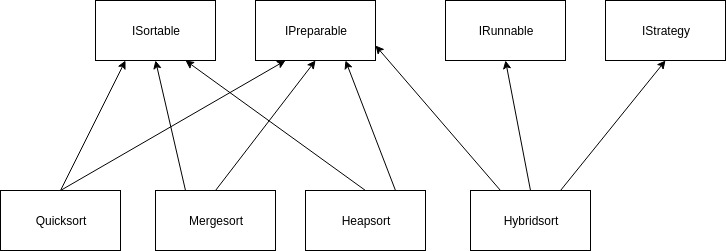
\includegraphics[width=0.8\textwidth]{diagrams/Hybrid_diagram.jpg}}
	\quad
	\caption{Diagram}
\end{figure}

\newpage
\section{Wykresy}

\subsection{Wybrane przypadki dla danych algorytmów sortowania}

\begin{figure}[ht]
	\centering
	\subfloat[Quicksort]{\label{odnosnik}
		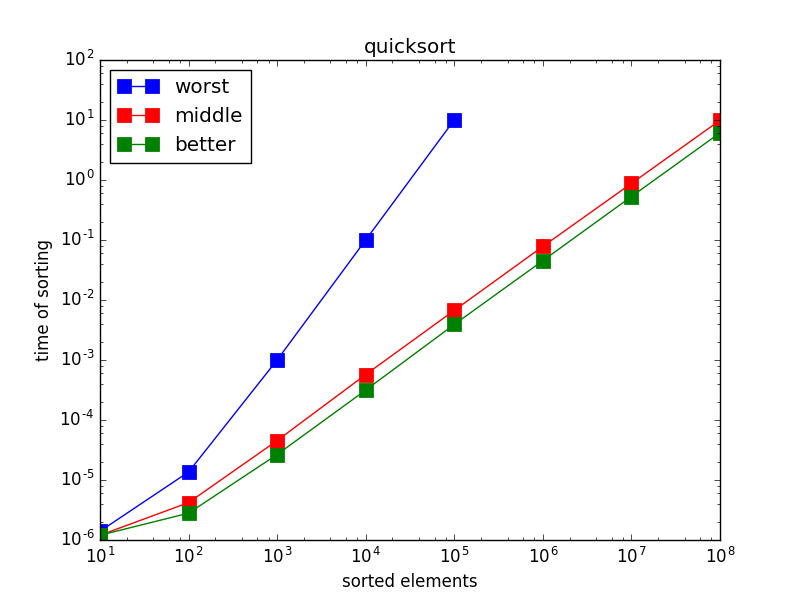
\includegraphics[width=0.6\textwidth]{images/quicksort_every_case.png}}
	\quad
	\caption{Przypadki dla algorytmu sortowania Quicksort}
\end{figure}

\begin{figure}[ht]
	\centering
	\subfloat[Mergesort]{\label{odnosnik}
		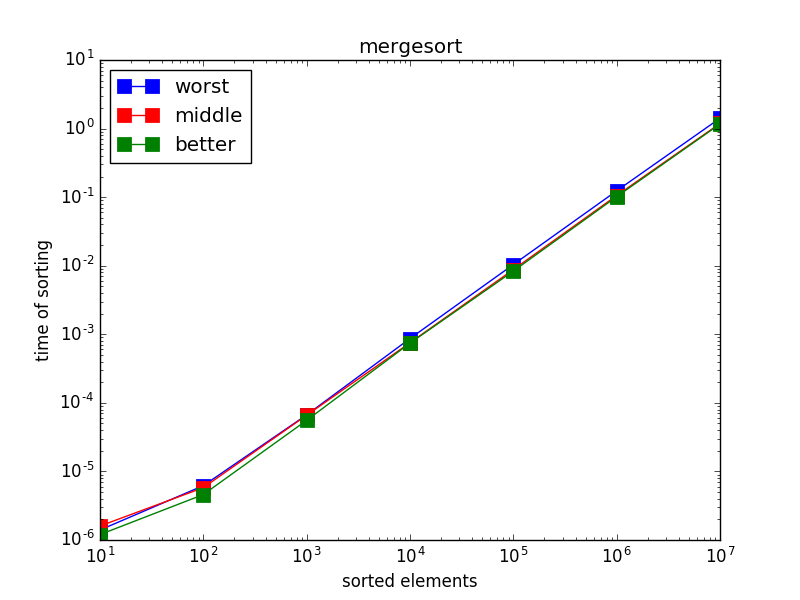
\includegraphics[width=0.6\textwidth]{images/mergesort_every_case.png}}
	\quad
	\caption{Przypadki dla algorytmu sortowania Mergesort}
\end{figure}

\begin{figure}[ht]
	\centering
	\subfloat[Heapsort]{\label{odnosnik}
		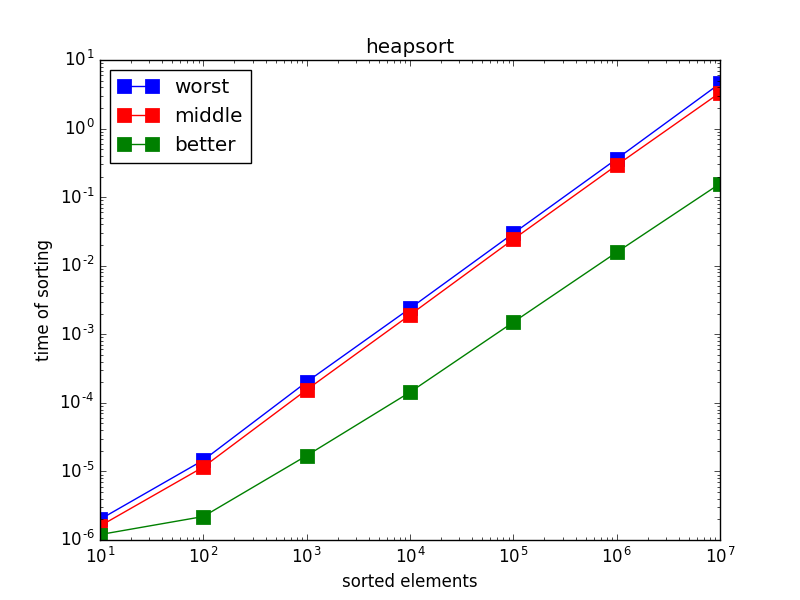
\includegraphics[width=0.6\textwidth]{images/heapsort_every_case.png}}
	\quad
	\caption{Przypadki dla algorytmu sortowania Heapsort}
\end{figure}

\newpage	
\subsection{Wybrane przypadki dla wszystkich algorytmów sortowania}	
	
\begin{figure}[ht]
	\centering
	\subfloat[worst-case]{\label{odnosnik}
		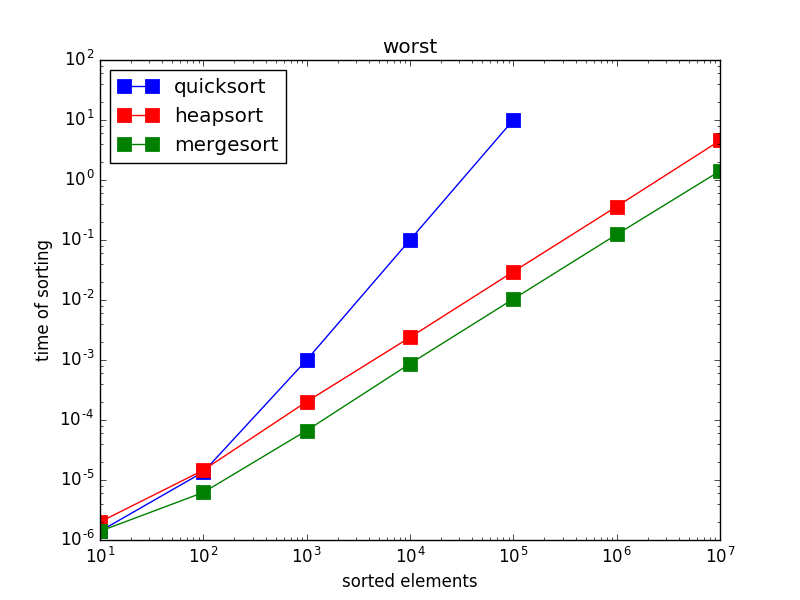
\includegraphics[width=0.6\textwidth]{images/worst_every_case.png}}
	\quad
	\caption{Przypadki pesymistyczne dla wszystkich algorytmów sortowania}
\end{figure}

\newpage
\begin{figure}[ht]
	\centering
	\subfloat[normal-case]{\label{odnosnik}
		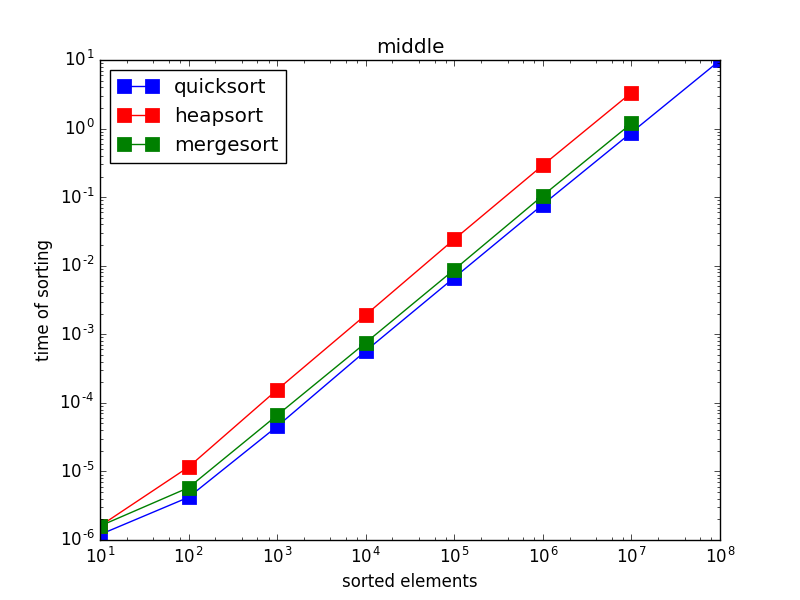
\includegraphics[width=0.6\textwidth]{images/middle_every_case.png}}
	\quad
	\caption{Przypadki normalne dla wszystkich algorytmów sortowania}
\end{figure}

\begin{figure}[ht]
	\centering
	\subfloat[the best-case]{\label{odnosnik}
		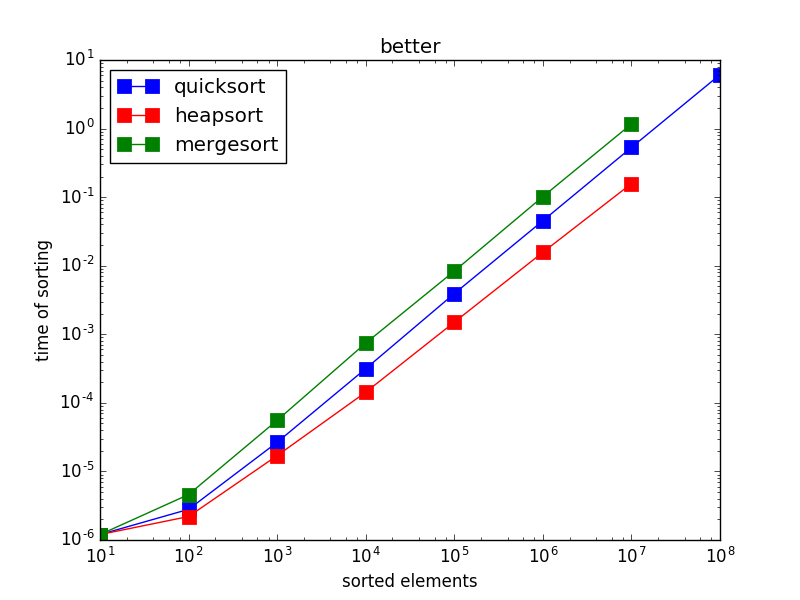
\includegraphics[width=0.6\textwidth]{images/better_every_case.png}}
	\quad
	\caption{Przypadki optymistyczne dla wszystkich algorytmów sortowania}
\end{figure}

\newpage
\section{Tabelki}

\subsection{Quicksort}

\subsubsection{Przypadek optymistyczny}

\begin{table}[htb]
    \centering
    \label{table:tablename}
	\csvautobooktabular{data_from_quicksort_better.csv}
	\quad
\end{table}

\subsubsection{Przypadek normalny}

\begin{table}[htb]
    \centering
    \label{table:tablename}
	\csvautobooktabular{data_from_quicksort_middle.csv}
	\quad
\end{table}

\subsubsection{Przypadek pesymistyczny}

\begin{table}[htb]
    \centering
    \label{table:tablename}
	\csvautobooktabular{data_from_quicksort_worst.csv}
	\quad
\end{table}

\newpage
\subsection{Mergesort}

\subsubsection{Przypadek optymistyczny}

\begin{table}[htb]
    \centering
    \label{table:tablename}
	\csvautobooktabular{data_from_mergesort_better.csv}
	\quad
\end{table}

\subsubsection{Przypadek normalny}

\begin{table}[htb]
    \centering
    \label{table:tablename}
	\csvautobooktabular{data_from_mergesort_middle.csv}
	\quad
\end{table}

\subsubsection{Przypadek pesymistyczny}

\begin{table}[htb]
    \centering
    \label{table:tablename}
	\csvautobooktabular{data_from_mergesort_worst.csv}
	\quad
\end{table}

\newpage
\subsection{Heapsort}

\subsubsection{Przypadek optymistyczny}

\begin{table}[htb]
    \centering
    \label{table:tablename}
	\csvautobooktabular{data_from_heapsort_better.csv}
	\quad
\end{table}

\subsubsection{Przypadek normalny}

\begin{table}[htb]
    \centering
    \label{table:tablename}
	\csvautobooktabular{data_from_heapsort_middle.csv}
	\quad
\end{table}

\subsubsection{Przypadek pesymistyczny}

\begin{table}[htb]
    \centering
    \label{table:tablename}
	\csvautobooktabular{data_from_heapsort_worst.csv}
	\quad
\end{table}

\newpage
\section{Wnioski}
\textbf{Sortowanie Szybkie(QuickSort)} charakteryzuje się oczekiwaną złożonością obliczeniową O(n lg n). W przypadku optymistycznym ilość porównań wykonywanych we wszystkich operacjach wynosi około n(lgn+1), co oznacza że złóżoność obliczeniowa wynosi O(n lg n). W przypadku średnim, gdy liczby są ułożone losowo złożoność obliczeniowa podobna jest do O(n lg n). W przypadku pesymistycznym z kolei wynosic O($n^2$). Quicksort najbardziej sprawdza się do sortowania dużych ilości elementów.\\

\textbf{Sortowanie przez scalanie(MergeSort)} w przypadku optymistycznym i średnim charakteryzuje się złożonością obliczeniową O(n lg n). W przypadku pesymistycznym złożoność ta również wynosi O(n lg n).Jednak algorytm sortowania przez scalanie nie stosuje się w przypadku dużych ilości danych, ze zwględu na wykorzystanie dodatkowego miejsca w pamięci podczas scalania tablic. Sprawdza się najlepiej w przypadkach pesymistycznych.\\

\textbf{Sortowanie przez kopcowanie(HeapSort)} charakteryzuje sie oczekiwaną złożonością
obliczeniową O(n lg n). W przypadku optymistycznym, średnim i pesymistycznym wynosi ona O(n lg n).Heapsort jest gorszy od QuickSorta, jednak w przypadkach pesymistycznych sprawia się lepiej. Wolniejszy od MergeSorta. Najlepiej sprawdza się w optymalnych przypadkach.\\

Wyniki Naszych badań związanych z obliczaniem złożoności czasowej poszczególnych algorytmów w różnych przypadkach są podobne do tych w ksiązkach i w internecie, co sugeruje poprawną implementacje i sposób działania algorytmów.

\section{Wykorzystane biblioteki}
Python:
\begin{enumerate}
	\item numpy
	\item matplotlib.pyplot
	\item os
	\item pathlib
\end{enumerate}

\end{document}
	